\chapter{Architettura}

In questo capitolo verranno descritte le scelte architetturali e implementative che stanno alla base del contributo di questa tesi al progetto IoE. 

Lo scenario legato alla mobilità elettrica veicolare è caratterizzato dalla presenza di diversi domini applicativi, piattaforme e parti interessate i quali necessitano di comunicare in modo unificato e trasparente. A tal fine è stato utilizzato il progetto Smart-M3 (\cite{tullio2011}) che è il cuore della nostra architettura. Appoggiandosi sulle tecnologie tipiche del \emph{Semantic Web} Smart-M3 assicura l'interoperabilità tra gli attori in gioco. 

In particolare vedremo come possono coesistere elementi reali ed elementi simulati e come il passaggio dall'uno all'altro sia assolutamente trasparente a tutti i componenti del sistema grazie all'uso di tecnologie ontology-based.

\section{Smart-M3}

Prima di parlare dei componenti strettamente legati a questo progetto è doveroso fare un introduzione alla tecnologia che fa da collante tra di essi ovvero Smart-M3. Capire come funziona Smart-M3 e quali sono i suoi principi è fondamentale al fine di comprendere a fondo il resto di questo documento.

M3 è un architettura middleware per consentire L'interoperabilità delle informazioni in maniera cross-domain, multi-vendor, multi-device, multi-piattaforma (\cite{smart2013}). Smart-M3 è la sua prima implementazione Open Source, proposta da SOFIA, un Progetto Europeo (2009-11), appartenente al framework ARTEMIS. 
La piattaforma implementa il disaccoppiamento tra produttori e consumatori di informazione. In questa architettura tutti gli attori (sensori, dispositivi, servizi, attuatori ecc..) cooperano attraverso un database RDF che è lo standard deciso dal World Wide Web Consortium per la descrizione di informazioni e concetti. L'interoperabilità è resa possibile da un modello di dati condiviso che si basa su tecnologie tipiche del Semantic Web.

Il Semantic Web è un framework sviluppato dal World Wide Web Consortium per consentire la condivisione e il riutilizzo dei dati attraverso  applicazioni, aziende e comunità eterogenee.

La figura ~\ref{fig:smart-m3} mostra il funzionamento dell'architettura M3. Il "legacy gate" è un interfaccia con il mondo esterno e di essi ne possono coesistere innumerevoli in un architettura M3.

\begin{figure}[H]
	\centering
	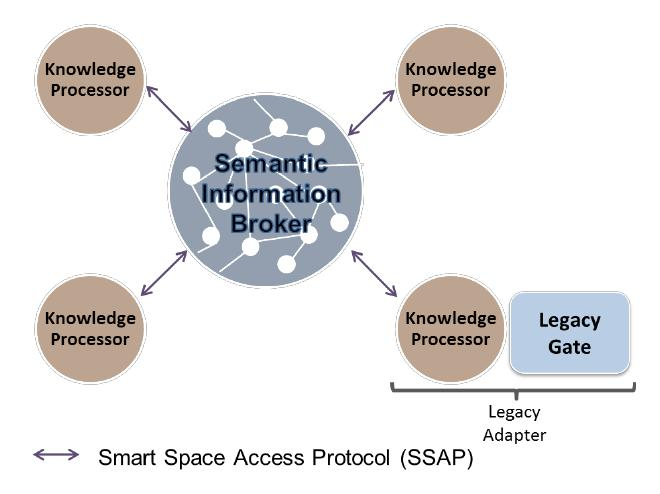
\includegraphics[width=0.5\textwidth]{assets/smart-m3.jpg}
	\caption{Architettura Smart-M3}
	\label{fig:smart-m3}
\end{figure}

\subsection{Semantic Information Broker}\label{subsec:sib}

Il \emph{Semantic Information Broker} (SIB) è l'entità responsabile della conservazione e della gestione delle informazioni condivise nell'architettura M3. Gli agenti Software che si scambiano le informazioni vengono chiamati \emph{Knowledge Processors} (KPs). L'accesso alla SIB da parte dei KP avviene attraverso lo \emph{Smart Space Access Protocol}  (SSAP), esso consiste in messaggi XML scambiati attraverso socket TCP/IP. Vengono fornite API che implementano il protocollo SSAP in diversi linguaggi.

Il SIB è un architettura a 5 livelli (\cite{smart2010}) come mostrato in figura ~\ref{fig:sib-architecture}:

\begin{enumerate}
	\item \textbf{Transport}: Questo livello consiste in una o più comunicazioni di rete a livello di trasporto che permette al SIB di comunicare con diverse reti e architetture. Il livello di trasporto è collegato a quello sottostante tramite il DBus, rendendo possibile l'aggiunta e la rimozione di connettori a runtime.
	\item \label{enum:handling}\textbf{Operation Handling}: A questo livello vengono gestite le operazioni del protocollo SSAP e ognuna di esse viene eseguita in un thread dedicato. Malgrado l'uso intensivo di thread possa degradare le performance la chiarezza di codice che ne consegue è stata ritenuta più importante.
	\item \label{enum:graph}\textbf{Graph Operations}: Questo livello gestisce le operazioni di inserimento, rimozione e query dal database RDF come richiesto dal livello ~\ref{enum:handling}. Viene eseguito all'interno di un singolo thread che schedula ed esegue le richieste provenienti dai thread che gestiscono le operazioni SSAP la quale comunicazione avviene tramite code asincrone.
	\item \textbf{Triple Operations}: A questo livello vengono gestite le operazioni SPARQL, WQL e le query basate su pattern-matching di triple RDF. Attualmente è implementato tramite Piglet, un database RDF che si appoggia ad SQL lite per la persistenza delle informazioni. Questo strato può essere tranquillamente cambiato a patto che si scriva il codice necessario ad interfacciare le operazioni a livello di grafo (~\ref{enum:graph}) con l'interfaccia fornita dal nuovo store RDF.
	\item \textbf{Persistent storage}: Quetso è il livello che assicura la persistenza dei dati.
\end{enumerate}

\subsection{I Knowledge Processor}

I Knowledge Processor (KP) sono le parti attive dell'architettura Smart-M3. Un KP interagisce con il SIB non direttamente tramite il protocollo SSAP ma tramite le Knowledge Processor Interface (KPI) ovvero delle librerie che lo implementano. Esse possono trovarsi a qualunque livello di astrazione ed essere scritte in qualunque linguaggio. Le funzioni messe a disposizione dal KPI in genere sono speculari alle operazioni del protocollo SSAP.

I KP sono quelle entità che forniscono, modificano e richiedono le informazioni le informazioni contenute nello smart-space. L'architettura dei KP è mostrata in figura ~\ref{fig:kp-architecture}.

\begin{figure}[H]
        \centering
        \begin{subfigure}[H]{0.5\textwidth}
                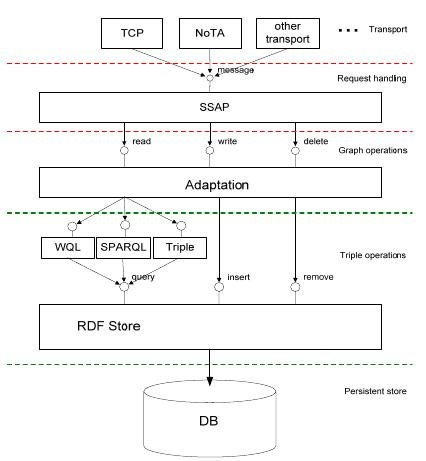
\includegraphics[width=\textwidth]{assets/sib-architecture.jpg}
                \caption{Architettura del SIB}
                \label{fig:sib-architecture}
        \end{subfigure}%
        \begin{subfigure}[H]{0.42\textwidth}
                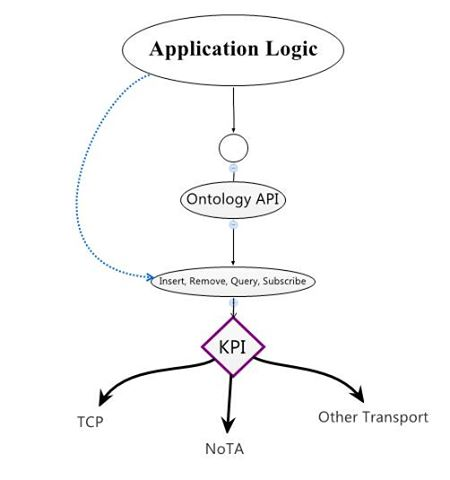
\includegraphics[width=\textwidth]{assets/kp-architecture.jpg}
                \caption{Architettura dei KP}
                \label{fig:kp-architecture}
        \end{subfigure}
        \caption{Architetture SIB e KP}
\end{figure}

\subsection{Le triple RDF}

Nell'architettura Smart-M3 le informazioni sono rappresentate in formato RDF (Resource Description Framework). In RDF le informazioni sono rappresentate come una tripletta \emph{soggetto, predicato, oggetto}. Le triple vengono memorizzate nel SIB e formano un grafo etichettato diretto il quale non necessariamente è un grafo connesso.

\subsection{Ontologie}

Mentre RDF fornisce il modello di dati standard per la rappresentazione delle informazioni, l'uso di un linguaggio ontologico è indispensabile per assegnare una semantica all'informazione. Linguaggi ontologici come RDFS e OWL forniscono un vocabolario comune. L'uso di una ontologia comune consente a tutti gli attori (uomini e macchine) di capire reciprocamente la semantica delle informazioni e di cooperare in simbiosi attraverso il SIB. Smart-M3 è agnostico rispetto all'ontologia e quindi consente agli sviluppatori di scegliere il modo migliore di modellare le informazioni al fine di soddisfare le esigenze funzionali del dominio applicativo indirizzato.

\subsection{Sottoscrizioni}

Un aspetto fondamentale di questa tecnologia è il meccanismo delle sottoscrizioni grazie al quale è possibile ricevere notifiche al variare di set di triple. Le sottoscrizioni sono determinanti nella nostra architettura perché, come vedremo più avanti (Sez. ~\ref{sec:protocol}), sono alla base dei protocolli di scambio dati tra i componenti del sistema.

\subsection{SPARQL}

SPARQL, si pronuncia sparkle, (acronimo ricorsivo di SPARQL Protocol and RDF Query Language) è il linguaggio standard de facto per interrogare dei dataset RDF. Come si può dedurre dal nome stesso SPARQL non è semplicemente un linguaggio di interrogazione di dati RDF, ma definisce anche il protocollo applicativo utilizzato per comunicare con le sorgenti RDF (si tratta di un binding su HTTP).

Così come SQL riflette, nella rappresentazione della query, il modello relazionale sottostante, allo stesso modo SPARQL basa la rappresentazione della query sul concetto di tripla e di grafo. Il meccanismo alla base della rappresentazione di una query e della ricerca della sua risposta è il graph matching. La query rappresenta un pattern di un grafo (RDF) e la risposta alla query sono tutte le triple (sotto-grafo) che fanno match con il pattern.

\subsection{Il protocollo SSAP}

L'SSAP (\emph{Smart Space Access Protocol}) è il protocollo con cui si comunica con il SIB. Il protocollo è session-based, i KP che vogliono comunicare con lo smart-space dovranno prima aderirvi con un operazione di Join prevista dall'SSAP. Il KP fornisce le sue credenziali nel messaggio di Join, il SIB esamina le credenziali e decide se accetare il KP o meno. Dopo l'operazione di Join, il KP può eseguire le altre operazioni. 
L'SSAP è il punto di integrazione principale dell'architettura Smart-M3. Le implementazioni di SIB e KP devono implementare tutte le operazioni del protocollo SSAP al fine di garantire l'interoperabilità.

Le operazioni supportate dal protocollo SSAP sono:

\begin{itemize}
	\item \textbf{JOIN}: Associa il KP allo smart-space solo se le credenziali verranno ritenute valide. Determina l'inizio della sessione.
	\item \textbf{LEAVE}: Determina il termine dell'associazione con lo smart-space e quindi la fine della sessione. Da questo momento in poi non potranno essere eseguite altre operazione di associazione allo smart-space.
	\item \textbf{INSERT}: Operazione atomica di inserzione di un Grafo, formato da triple RDF, nel SIB.
	\item \textbf{REMOVE}: Operazione atomica di rimozione di un Grafo, formato da triple RDF, nel SIB.
	\item \textbf{UPDATE}: Operazione atomica di aggiornamento di un Grafo, formato da triple RDF, nel SIB. In realtà si tratta di una combinazione di DELETE e INSERT eseguita in modo atomico dove l'operazione di DELETE viene eseguita per prima.\textsl{•}
	\item \textbf{QUERY}: Richiesta di informazioni contenute nel SIB attraverso una delle modalità supportate.
	\item \textbf{SUBSCRIBE}: Sottoscrizione a un set di triple contenute nel SIB. Il KP riceve una notifica quando avviene un cambiamento su una di queste triple.
	\item \textbf{UNSUBSCRIBE}: Cancella una sottoscrizione.
\end{itemize}

%\begin{figure}
%	\centering
%	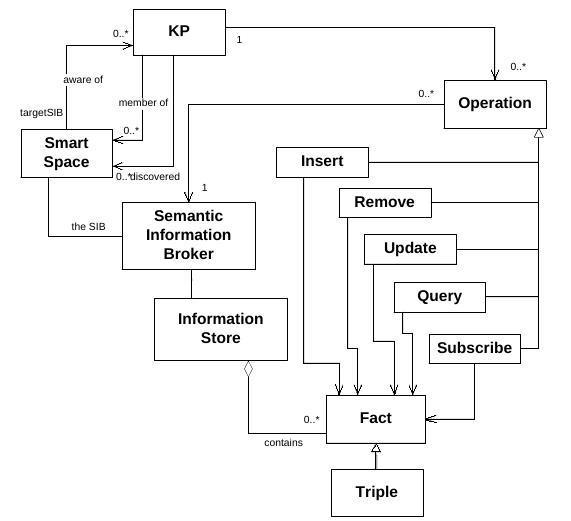
\includegraphics[width=0.5\textwidth]{assets/smart-m3-domain.jpg}
%	\caption{Smart-M3 modello di dominio}
%	\label{fig:smart-m3-domain}
%\end{figure}

\section{Il Modello Ontologico}

In questa sezione verrà spiegato come sono stati modellati i dati attraverso un ontologia. Il modello ontologico è stato ereditato dalla progetto di Tesi di \emph{Federico Montori} (\cite{montori2012}). Io ho contribuito espandendolo al fine di adattarlo ai nuovi requisiti funzionali sorti durante lo sviluppo del progetto. Verranno quindi mostrate gli aspetti dell'ontologia necessari a comprendere il resto della trattazione e verranno approfondite le modifiche da me apportate.

\subsection{Introduzione}

L'ontologia è definibile come una rappresentazione formale ed esplicita di una concettualizzazione condivisa di un dominio di interesse.

L'ontologia presenta le seguenti proprietà:

\begin{itemize}
	\item \textbf{Rappresentazione Formale}: Utilizza pertanto un linguaggio logico processabile da elaboratori.
	\item \textbf{Esplicita}: Cioè non ambigua e tale da chiarire ogni assunzione fatta.
	\item \textbf{Concettuale}: È una concettualizzazione cioè una vista astratta e semplificata del dominio di interesse
	\item \textbf{Condivisa}: Determinata dal consenso di una pluralità il più ampia possibile di soggetti.
\end{itemize}

Lo scopo delle ontologie è quindi descrivere delle basi di conoscenze, effettuare delle deduzioni su di esse e integrarle tra le varie applicazioni. Per descrivere le ontologie viene utilizzato il linguaggio OWL (\emph{Ontology Web Language}) che è un estensione di RDF. È un linguaggio di markup per rappresentare esplicitamente significato e semantica di termini con vocabolari e relazioni tra gli stessi.

I linguaggi della famiglia OWL sono in grado di creare \emph{classe}, \emph{proprietà}, \emph{istanze} e le relative \emph{operazioni}.


\subsection{Classi di IoE}

Una classe è una collezione di oggetti che corrisponde alla descrizione logica di un concetto. Da una classe si possono creare un numero arbitrario di istanze mentre ad un istanza può corrispondere ad una, nessuna o molteplici classi.\newline
Una classe può essere sottoclasse di un'altra classe, ereditando le caratteristiche della super-classe. Tutte le classi sono sottoclasse di \code{owl:Thing}.

Nel modello di dati utilizzato in questo progetto si è cercato di tenere disaccoppiato il concetto di dato dalle altre entità fisiche. Ne consegue che tutte le entità fisiche sono sottoclassi dirette di \code{owl:Thing}, mentre le classi destinate a rappresentare i dati sono sottoclasse di \code{ioe:Data} che a sua volta è sottoclasse di \code{owl:Thing}.\newline
Nel resto di questo documento userò il prefisso \code{ioe:} come abbreviazione di \emph{http://www.m3.com/2012/05/m3/ioe-ontology.owl\#} che è il namespace scelto per l'ontologia. In generale userò questo prefisso per distinguere le classi dell'ontologia dalle classi Java che come vedremo nella sezione ~\ref{subsec:ioe-lib} hanno lo stesso nome essendo mapping diretto di quest'ultime.

\subsection{Sottoclassi di owl:Thing}

Come già accennato tutte le entità fisiche del nostro modello ontologico sono sottoclasse diretta di owl:Thing. Quellla mostrata di seguito è una lista delle Classi utilizzate in questo progetto, vengono omesse quelle che sono attualmente irrilevanti o inutilizzate.

\begin{itemize}
	\item \textbf{Person}: Questa classe rappresenta il concetto di persona. Ad ogni persona possono essere associati diversi veicoli (Vehicle), diverse richieste di ricarica (Reservation), nonché una storia delle ricariche effettuate (Recharge). Il concetto di persona viene utilizzato ai fini di autenticazione e in un futuro potrà essere determinante ai fini della fatturazione che il provider energetico eseguirà in seguito alle ricariche.
	\item \textbf{Vehicle}: Rappresenta il concetto di Veicolo Elettrico, siccome i veicoli non elettrici sono irrilevanti al fine di questa trattazione è stata usata direttamente questa classe allo scopo. Ad ogni veicolo sono ovviamente associati i dati della batteria (BatteryData) che verranno trattati nella sezione relativa alle sottoclassi di \code{ioe:Data} (~\ref{subsec:ioe-data});
	\item \textbf{GridConnectionPoint}: Il \emph{Grid Connection Pointer} (GCP) è la stazione di ricarica. Esso contiene almeno un EVSE che invece rappresenta la colonnina dove ci si ricarica effettivamente. Il rapporto tra un GCP e gli EVSE è lo stesso che intercorre tra una stazione di rifornimento e le pompe di benzina. 
	\item \textbf{EVSE}: Il \emph{Electrical Vehicle Supply Equipment} è il punto in cui il veicolo si connette alla rete elettrica. Una volta connesso può sia ricaricare la sua batteria che cedere energia alla smart-grid. Un EVSE ha diversi connettori (Connector) per adattarsi ai vari tipi di presa posseduti dai veicoli elettrici. Inoltre, ogni EVSE, ha una lista di prenotazioni associate.
	\item \textbf{ChargeProfile}: È l'insieme dei parametri che caratterizzano il profilo energetico di un EVSE in un determinato istante. I parametri attualmente sono: potenza, orario di validità del profilo stesso e prezzo per unità di energia (in genere 1 kWh). Ovviamente può essere attivo un solo ChargeProfile alla volta e il variare di quest'ultimi può essere determinato da fasce orarie proprio come avviene per l'energia elettrica casalinga.
	\item \textbf{Connector}: È il connettore di ricarica ovvero il punto i contatto tra l'EVSE e l'EV. Ogni EVSE può avere diversi connettori al fine di poter essere compatibile con il maggior numero di veicoli possibile. Malgrado negli usa si stia cercando di introdurre uno standard a riguardo ormai esistono diversi tipi di connettori. 
	\item \textbf{ChargeRequest}: Richiesta di ricarica. Viene istanziata quando un utente necessita di creare una prenotazione e al suo interno sono contenuti tutti i parametri necessari a descriverla. Fa parte del protocollo di richiesta di prenotazione discusso nella sezione ~\ref{sec:protocol}. Mentre un approfondimento sulla sua struttura è trattato nella sezione ~\ref{subsubsec:chargerequest}.
	\item \textbf{ChargeResponse}: È la risposta fornita dal servizio cittadino a seguito della richiesta di prenotazione. Al suo interno contiene un riferimento alla richiesta (ChargeRequest) da cui è stata generata e una lista di opzioni di ricarica che aderiscono alla richiesta dell'utente (ChargeOption).
	\item \textbf{ChargeOption}: Fa parte della risposta(ChargeResponse) che il servizio cittadino da all'utente in seguito a una richiesta di prenotazione (ChargeRequest). Contiene i parametri di ricarica come EVSE, orario e prezzo. 
	\item \textbf{Currency}: Rappresenta una valuta relativa a un prezzo. Alcune sue istanze sono state inserte direttamente nell'ontologia (\code{ioe:Euro}, \code{ioe:Dollar} ecc..);
	\item \textbf{Reservation}: Se il protocollo di richiesta di prenotazione va a buon fine verrà creata un istanza di questa classe che indica che l'EVSE a cui è associata è occupato per un determinato periodo di tempo. 
	\item \textbf{ReservationList}: Lista di prenotazioni associate ad un EVSE. Ogni EVSE può avere un unica lista di prenotazioni associata.
	\item \textbf{ReservationRetire}: Classe che denota la volontà dell'utente di ritirare una prenotazione.
	\item \textbf{Recharge}: Quando un utente, in seguito a una prenotazione, termina di ricaricarsi, inserita questa entità ad esso associato. Denota l'avvenuta ricarica è può essere utile per tener traccia dell'attività dell'utente nonché per fare statistiche.
	\item \textbf{UnityOfMeasure}: Rappresenta l'unità di misura per i dati del progetto. Deve esserne associata una ad ogni sottoclasse di \code{ioe:Data}. Attualmente sono hardcoded all'interno dell'ontologia (\code{ioe:Watt}, \code{ioe:Volt} ecc..) 	
	\item \textbf{Data}: Questa classe rappresenta il concetto di dato misurabile e ogni sua sottoclasse sarà caratterizzata da un valore e da un unità di misura.
\end{itemize}

\subsection{Sottoclassi di ioe:Data}\label{subsec:ioe-data}


\subsection{Modifiche apportate all'ontologia}

\subsubsection{ChargeRequest}\label{subsubsec:chargerequest}

\subsubsection{ChargeRequest}\label{subsubsec:chargeresponse}